\section{Simulation}
\begin{frame} {Parameters}
    \begin{figure}
        \centering
        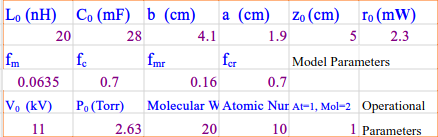
\includegraphics[width=0.7\textwidth]{figures/parameters.png}
        \caption{Input Parameters}
        \label{fig:parameters}
    \end{figure}
    \begin{itemize}
        \item The parameters are set to match the device NX2.
        \item Bank parameters, $L_0$, $C_0$ and stray circuit resistance $r_0$.
        \item Tube parameters $b$, $a$ and $z_0$.
        \item Operational parameters $V_0$ and $P_0$ and the fill gas.
    \end{itemize}
\end{frame}

\begin{frame} {Parameters - Continue}
    \begin{figure}
        \centering
        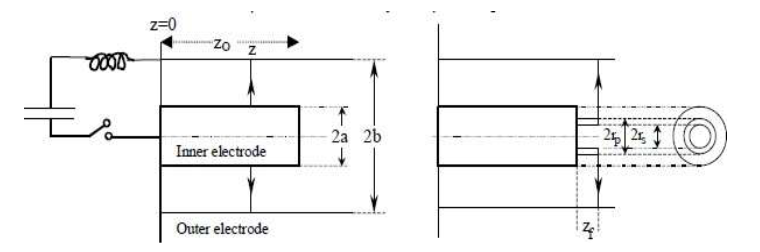
\includegraphics[width=\textwidth]{figures/dpf-device.png}
        \caption{DPF device.}
        \label{fig:dpf-device}
    \end{figure}
\end{frame}

\begin{frame} {Discharge Current}
    \begin{figure}
        \centering
        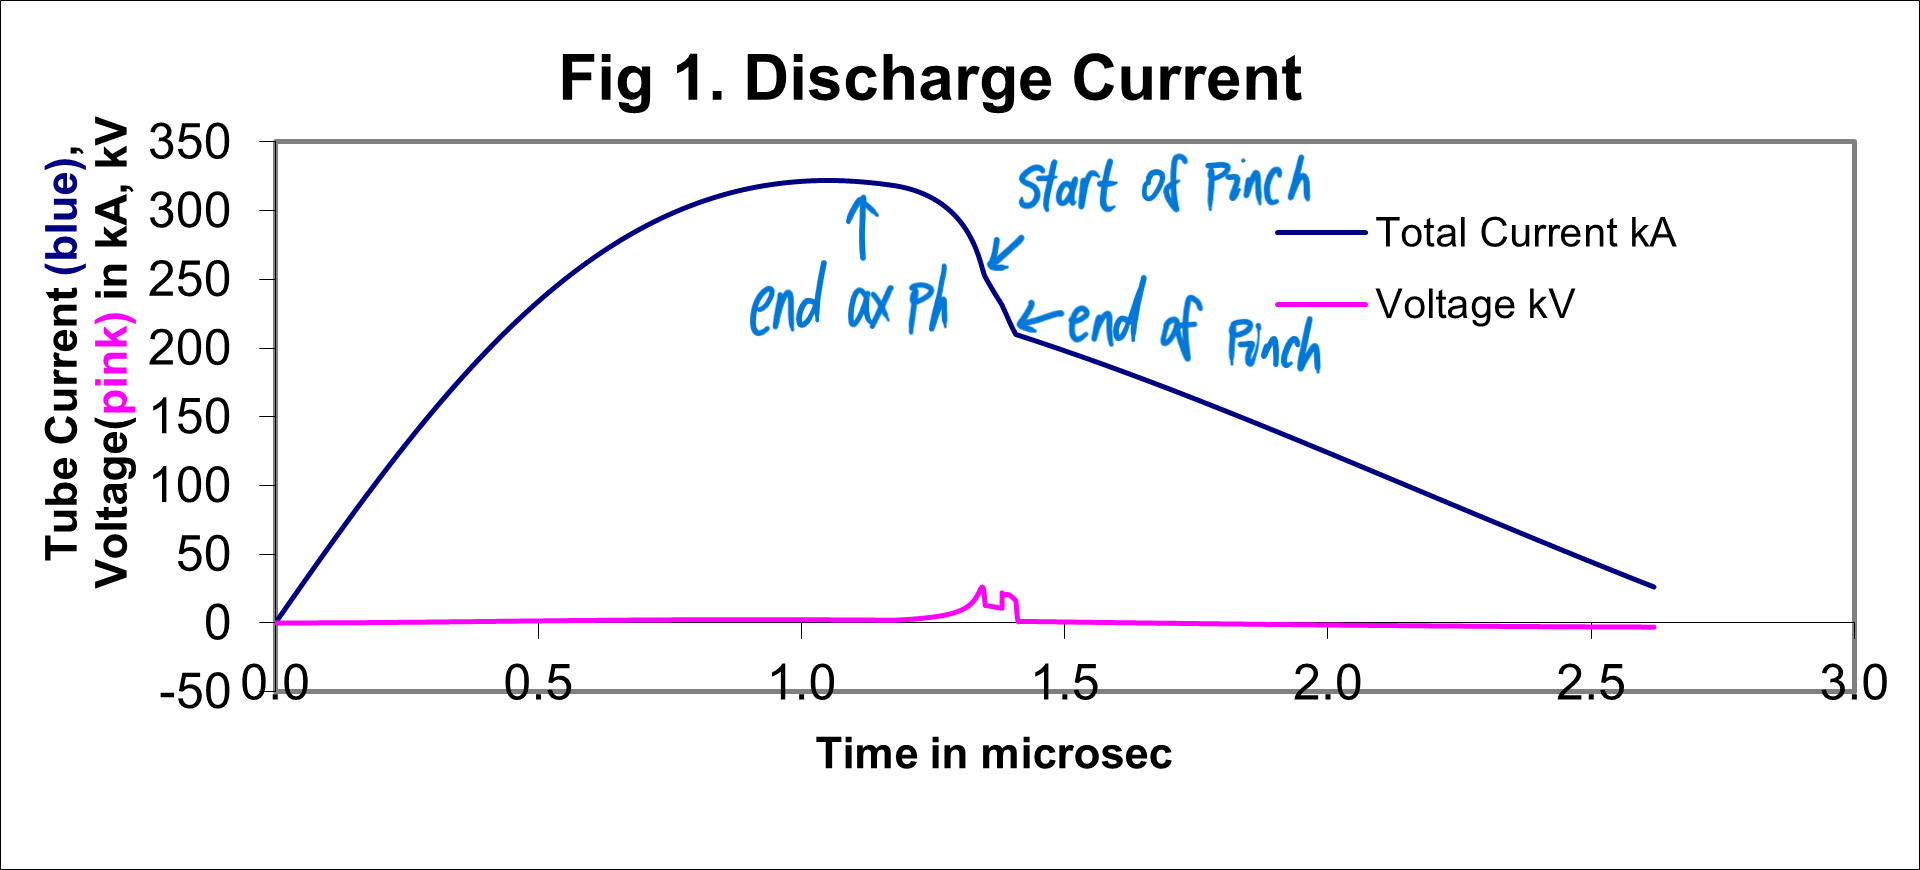
\includegraphics[width=0.7\textwidth]{figures/figure1.png}
        \caption{Discharge Current}
        \label{fig:discharge-Current}
    \end{figure}
    \begin{itemize}
        \item Axial phase ends after the discharge current reaches its peak (1.17\unit{\micro\s}).
        \item As the radial phase starts, the discharge current decreases.
        \item The pinch starts at 1.38\unit{\micro\s}.
        \item Then at 1.41\unit{\micro\s} the radial phase ends, also the pinch ends.
    \end{itemize}
\end{frame}

\begin{frame} {5-Point Fitting}
    \begin{figure}
        \centering
        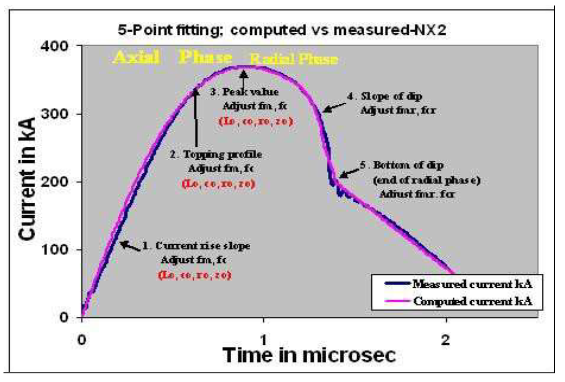
\includegraphics[width=0.5\textwidth]{figures/5-point-fitting.png}
        \caption{\scriptsize The 5-point fitting of computed current trace to measured (reference) current trace. Point 1 is the current rise slope. Point 2 is the topping profile. Point 3 is the peak value of the current. Point 4 is the slope of the current dip. Point 5 is the bottom of the current dip. Fitting is done up to point 5 only. Further agreement or divergence of the computed trace with/from the measured trace is only incidental and not considered to be important.}
        \label{fig:5-point-fitting}
    \end{figure}
    \begin{itemize}
        \item By fitting the 5 features, we are able to obtained the fitted model parameters: $f_m, f_c, f_{mr}$, and $f_{cr}$.
    \end{itemize}
\end{frame}

\begin{frame} {Speed of Current Sheet}
    \begin{figure}
        \centering
        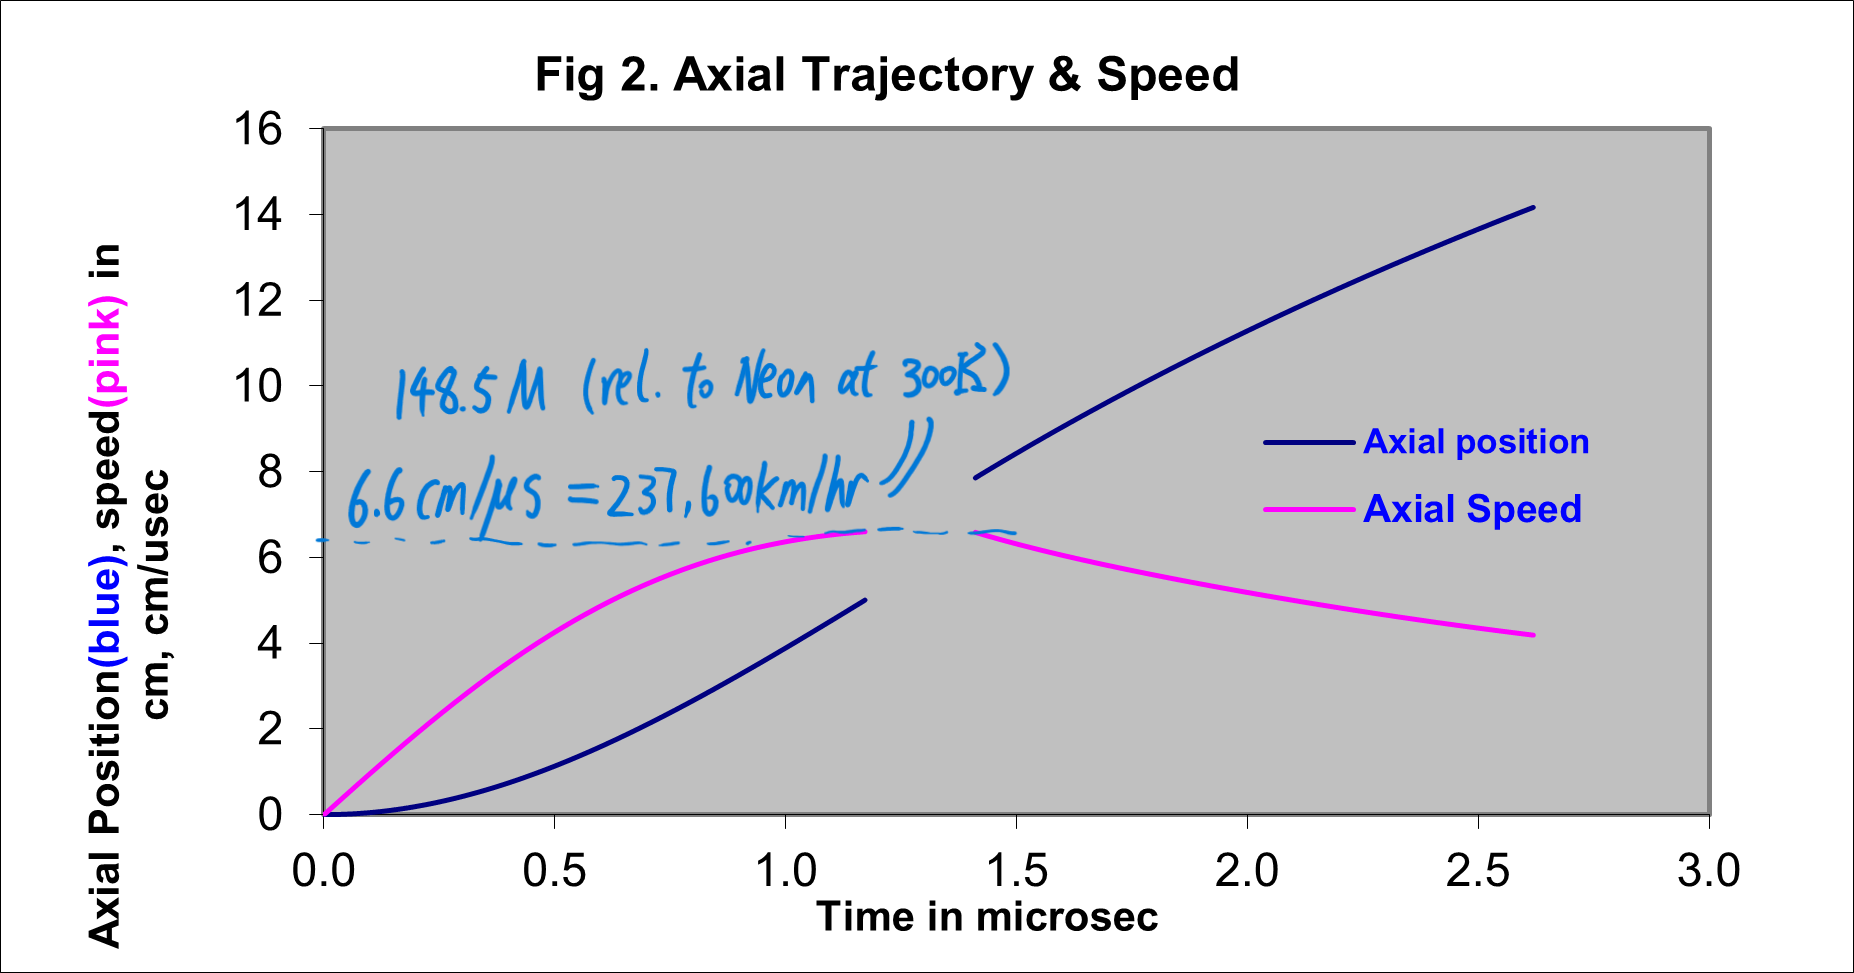
\includegraphics[width=0.7\textwidth]{figures/figure2.png}
        \caption{Axial Speed of the current sheet.}
        \label{fig:axial-speed}
    \end{figure}
    \begin{itemize}
        \item The speed of current sheet is fast.
        \item The speed of sound of Neon is 1500\unit{\kilo\m/\hour}. The Mach number is therefore 150M.
    \end{itemize}
\end{frame}

\begin{frame} {Radial Position}
    \begin{figure}
        \centering
        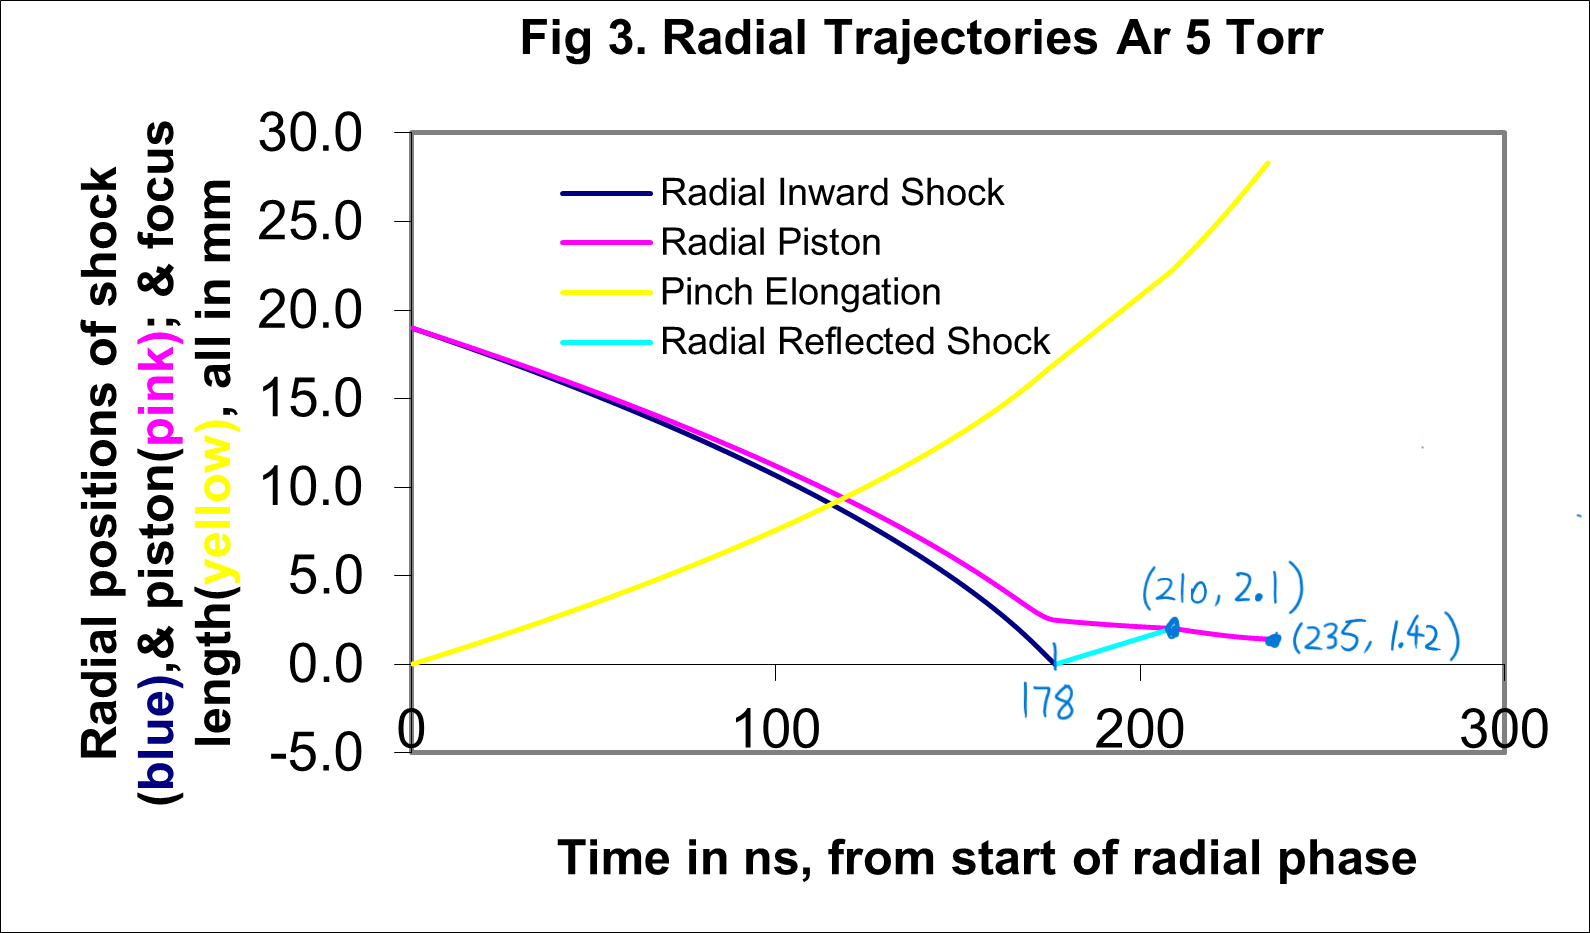
\includegraphics[width=0.55\textwidth]{figures/figure3.png}
        \caption{Radial position of the plasma column starting from radial phase.}
        \label{fig:radial-position}
    \end{figure}
    \begin{itemize}
        \item In the radial inward shock phase, both inner and outer radius of the plasma column decreases.
        \item After 178\unit{\nano\s}, radial reflected shock phase starts and the inner radius of the plasma column increases.
        \item After 210\unit{\nano\s}, it enters slow compression phase and the plasma column will be compressed to its minimum radius.
    \end{itemize}
\end{frame}

\begin{frame} {Temperature}
    \begin{figure}
        \centering
        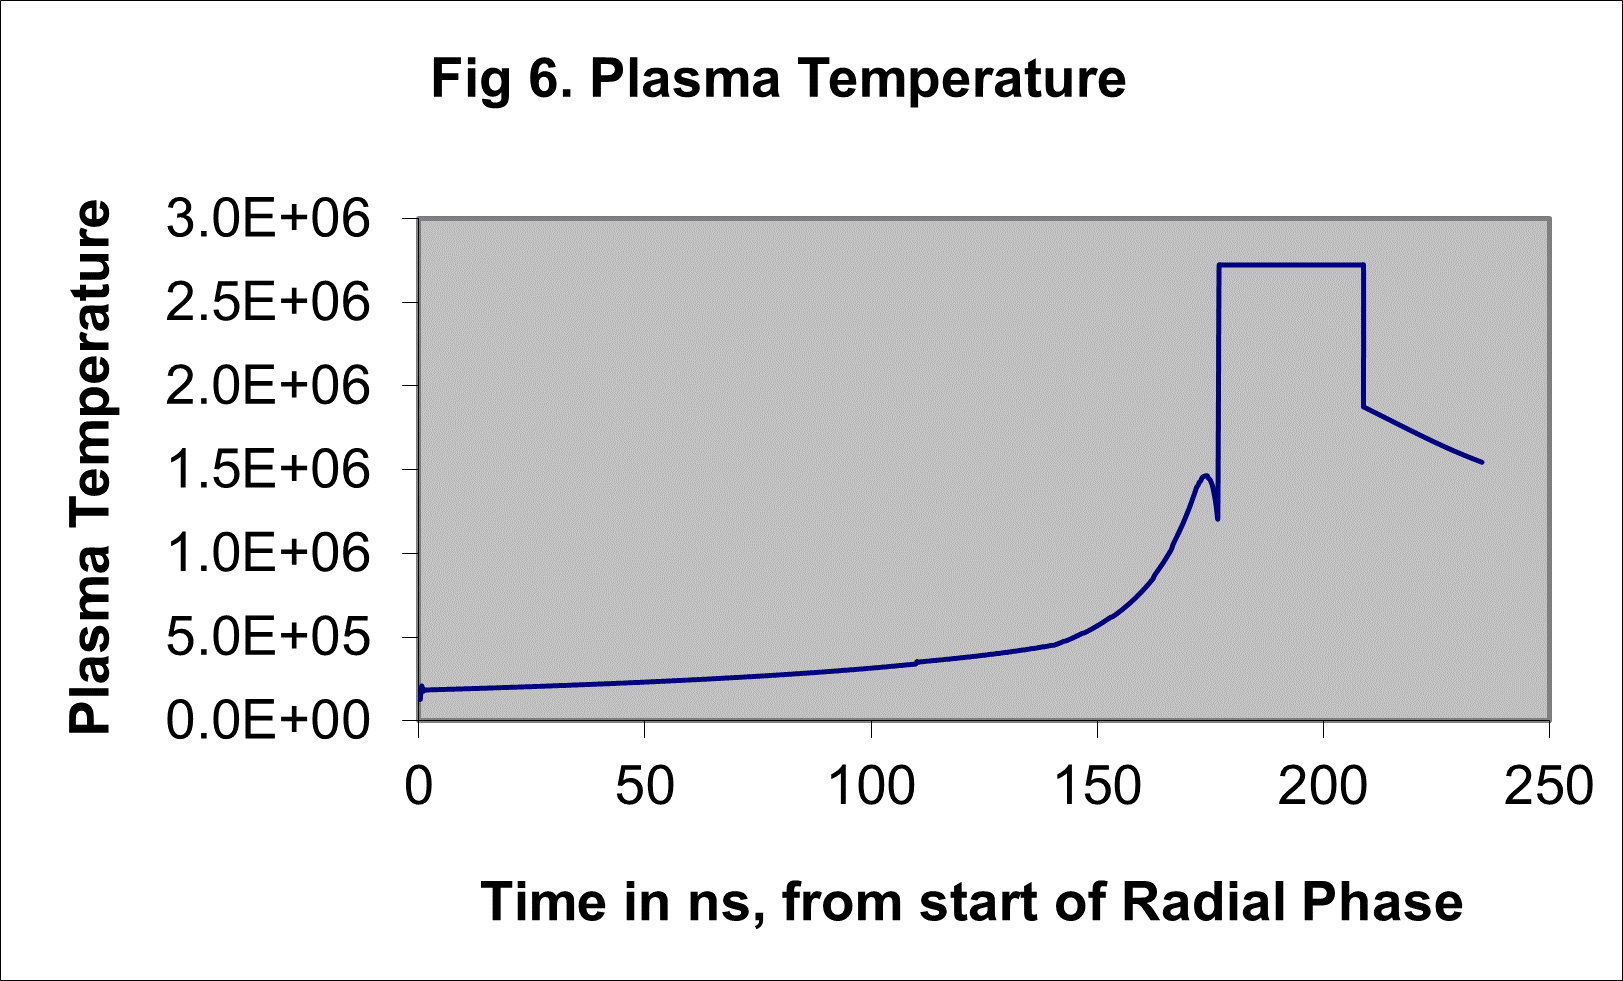
\includegraphics[width=0.6\textwidth]{figures/figure6.png}
        \caption{Plasma temperature in radial phase.}
        \label{fig:temperature}
    \end{figure}
    \begin{itemize}
        \item The plasma temperature raises during the radial inward shock phase.
        \item The plasma temperature reaches its maximum $2.72\times 10^6$K during the radial reflected shock phase.
        \item The temperature stays constant during the radial reflected shock phase.
    \end{itemize}
\end{frame}

\begin{frame} {Radiation}
    \begin{figure}
        \centering
        \begin{subfigure}{0.5\textwidth}
            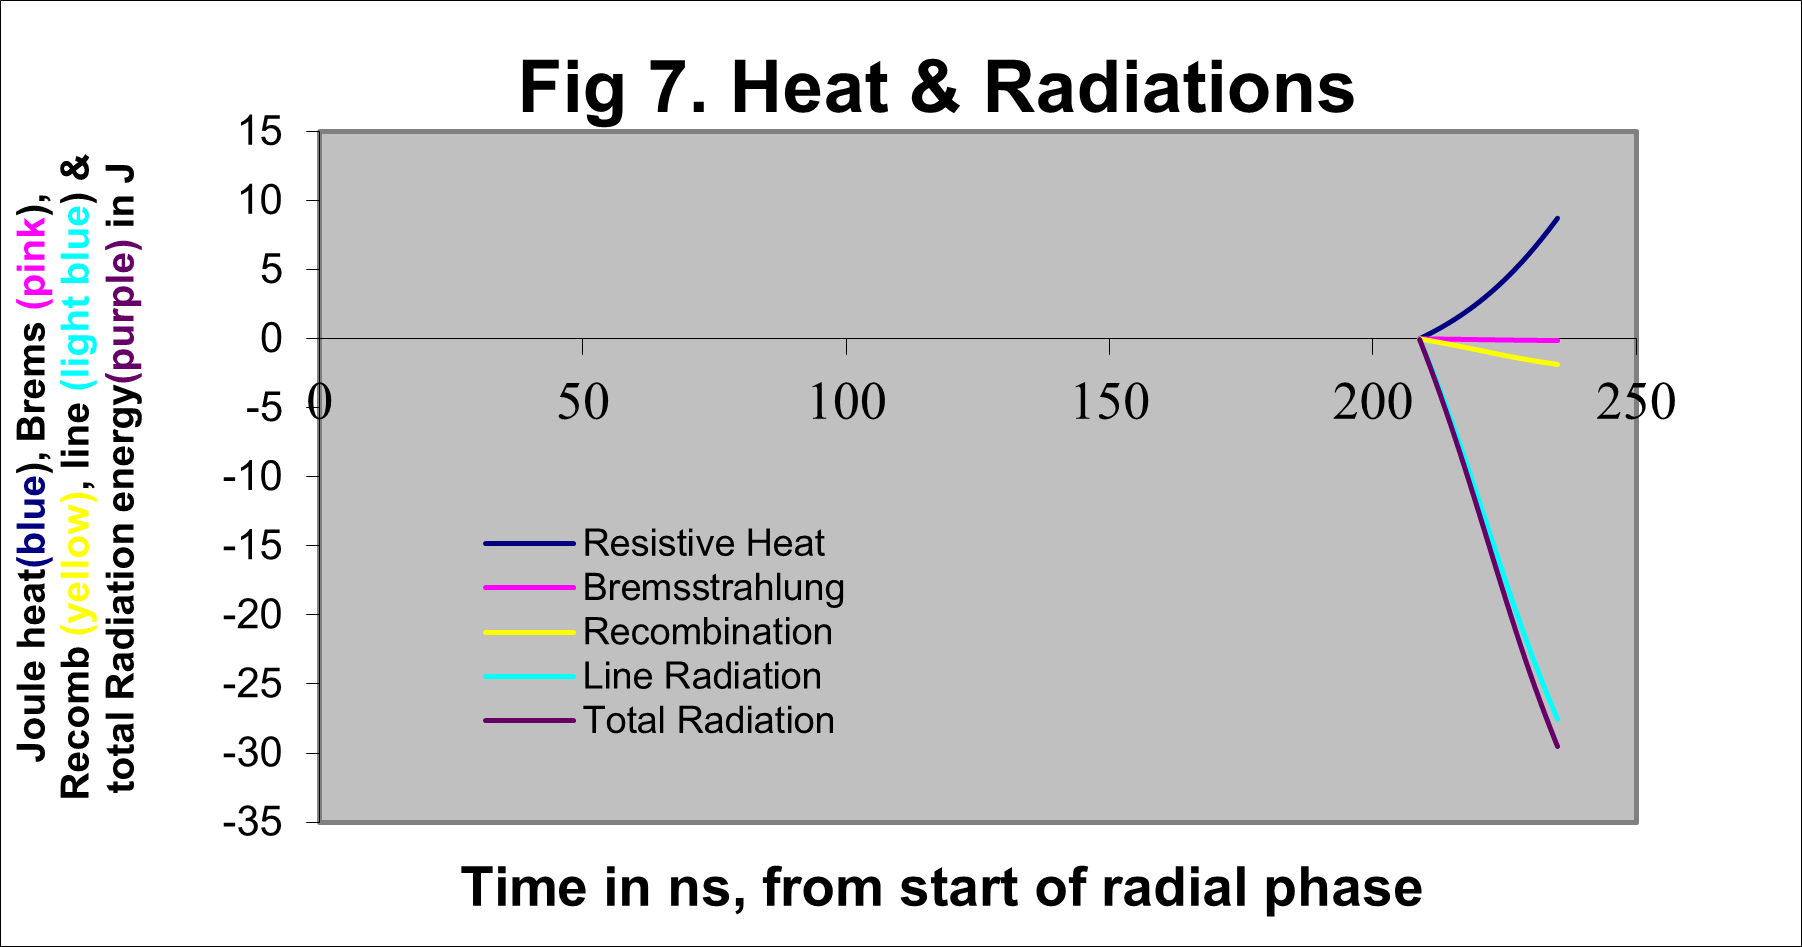
\includegraphics[width=\textwidth]{figures/figure7.png}
        \end{subfigure}%
        \begin{subfigure}{0.5\textwidth}
            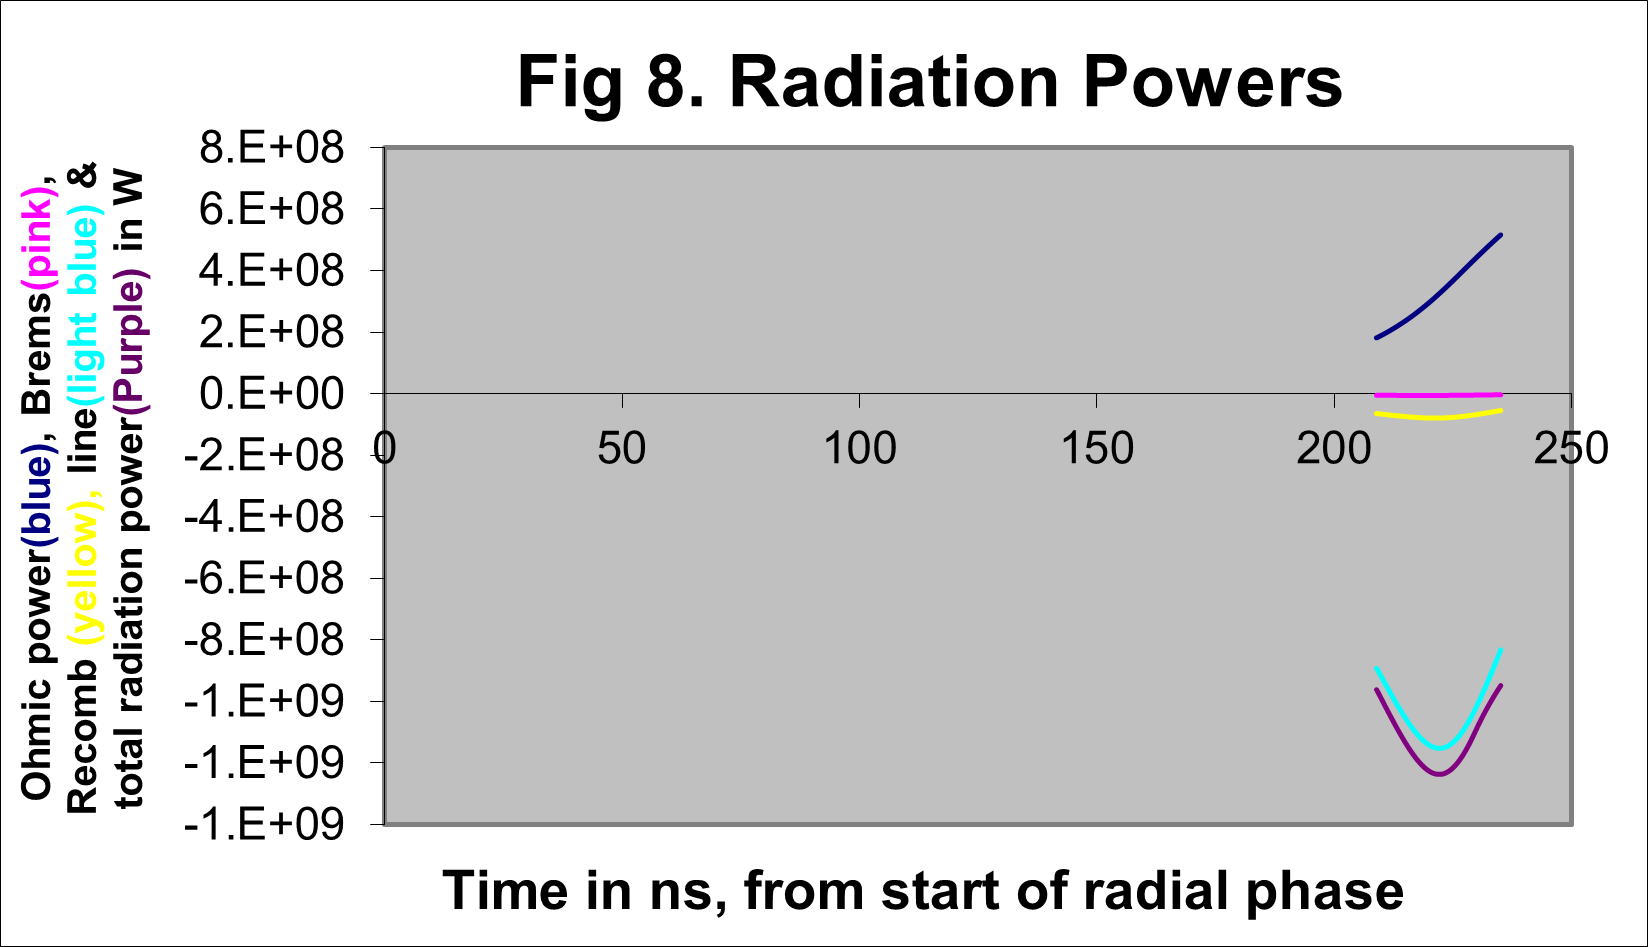
\includegraphics[width=0.9\textwidth]{figures/figure8.png}
        \end{subfigure}
        \caption{Radiation related graphs}
        \label{fig:radiation}
    \end{figure}
    \begin{itemize}
        \item Radiations starts after the pinch ends (plasmoid) is formed.
        \item Joule heating reached a maximum value of 8.73\unit{\J}
        \item Total radiation reached a maximum value of 30\unit{\J}
    \end{itemize}
\end{frame}